\documentclass[11pt]{article}
\usepackage{enumitem, listings}
\usepackage{xcolor}
\usepackage{caption}
\usepackage{subcaption}
\usepackage{amsgen,amsmath,amstext,amsbsy,amsopn,amssymb}
\usepackage{amsmath}
\usepackage{graphicx}
\usepackage{hyperref}
%New colors defined below
\definecolor{codegreen}{rgb}{0,0,1}
\definecolor{codegray}{rgb}{0.5,0.5,0.5}
\definecolor{codepurple}{rgb}{1,0.5,1}
\definecolor{backcolour}{rgb}{0.95,0.95,0.95}

%Code listing style named "mystyle"
\lstdefinestyle{mystyle}{
  backgroundcolor=\color{backcolour}, commentstyle=\color{codegreen},
  keywordstyle=\color{codegreen},
  numberstyle=\tiny\color{codegray},
  stringstyle=\color{codepurple},
  basicstyle=\ttfamily\footnotesize,
  breakatwhitespace=false,         
  breaklines=false,                 
  captionpos=b,                    
  keepspaces=false,                                   
  showspaces=false,                
  showstringspaces=false,
  showtabs=false,                  
  tabsize=2
}

%"mystyle" code listing set
\lstset{style=mystyle}

\RequirePackage{bm}

\textwidth 6.3in \textheight 8.8in \topmargin -0.5truein
\oddsidemargin .15truein
\parskip .1in
\renewcommand{\baselinestretch}{1.53}  % double spaced
\renewcommand{\abstractname}{Instructions}

\newtheorem{theorem}{\bf Theorem}

%----- bold fonts -----%

\newcommand{\ab}{\mathbf{a}}
\newcommand{\bbb}{\mathbf{b}}
\newcommand{\cbb}{\mathbf{c}}
\newcommand{\db}{\mathbf{d}}
\newcommand{\eb}{\mathbf{e}}
\newcommand{\fb}{\mathbf{f}}
\newcommand{\gb}{\mathbf{g}}
\newcommand{\hb}{\mathbf{h}}
\newcommand{\ib}{\mathbf{i}}
\newcommand{\jb}{\mathbf{j}}
\newcommand{\kb}{\mathbf{k}}
\newcommand{\lb}{\mathbf{l}}
\newcommand{\mb}{\mathbf{m}}
\newcommand{\nbb}{\mathbf{n}}
\newcommand{\ob}{\mathbf{o}}
\newcommand{\pb}{\mathbf{p}}
\newcommand{\qb}{\mathbf{q}}
\newcommand{\rb}{\mathbf{r}}
\newcommand{\sbb}{\mathbf{s}}
\newcommand{\tb}{\mathbf{t}}
\newcommand{\ub}{\mathbf{u}}
\newcommand{\vb}{\mathbf{v}}
\newcommand{\wb}{\mathbf{w}}
\newcommand{\xb}{\mathbf{x}}
\newcommand{\yb}{\mathbf{y}}
\newcommand{\zb}{\mathbf{z}}

\newcommand{\ba}{\bm{a}}
\newcommand{\bb}{\bm{b}}
\newcommand{\bc}{\bm{c}}
\newcommand{\bd}{\bm{d}}
\newcommand{\be}{\bm{e}}
\newcommand{\bbf}{\bm{f}}
\newcommand{\bg}{\bm{g}}
\newcommand{\bh}{\bm{h}}
\newcommand{\bi}{\bmf{i}}
\newcommand{\bj}{\bm{j}}
\newcommand{\bk}{\bm{k}}
\newcommand{\bl}{\bm{l}}
\newcommand{\bbm}{\bm{m}}
\newcommand{\bn}{\bm{n}}
\newcommand{\bo}{\bm{o}}
\newcommand{\bp}{\bm{p}}
\newcommand{\bq}{\bm{q}}
\newcommand{\br}{\bm{r}}
\newcommand{\bs}{\bm{s}}
\newcommand{\bt}{\bm{t}}
\newcommand{\bu}{\bm{u}}
\newcommand{\bv}{\bm{v}}
\newcommand{\bw}{\bm{w}}
\newcommand{\bx}{\bm{x}}
\newcommand{\by}{\bm{y}}
\newcommand{\bz}{\bm{z}}




\newcommand{\Ab}{\mathbf{A}}
\newcommand{\Bb}{\mathbf{B}}
\newcommand{\Cb}{\mathbf{C}}
\newcommand{\Db}{\mathbf{D}}
\newcommand{\Eb}{\mathbf{E}}
\newcommand{\Fb}{\mathbf{F}}
\newcommand{\Gb}{\mathbf{G}}
\newcommand{\Hb}{\mathbf{H}}
\newcommand{\Ib}{\mathbf{I}}
\newcommand{\Jb}{\mathbf{J}}
\newcommand{\Kb}{\mathbf{K}}
\newcommand{\Lb}{\mathbf{L}}
\newcommand{\Mb}{\mathbf{M}}
\newcommand{\Nb}{\mathbf{N}}
\newcommand{\Ob}{\mathbf{O}}
\newcommand{\Pb}{\mathbf{P}}
\newcommand{\Qb}{\mathbf{Q}}
\newcommand{\Rb}{\mathbf{R}}
\newcommand{\Sbb}{\mathbf{S}}
\newcommand{\Tb}{\mathbf{T}}
\newcommand{\Ub}{\mathbf{U}}
\newcommand{\Vb}{\mathbf{V}}
\newcommand{\Wb}{\mathbf{W}}
\newcommand{\Xb}{\mathbf{X}}
\newcommand{\Yb}{\mathbf{Y}}
\newcommand{\Zb}{\mathbf{Z}}

\newcommand{\bA}{\bm{A}}
\newcommand{\bB}{\bm{B}}
\newcommand{\bC}{\bm{C}}
\newcommand{\bD}{\bm{D}}
\newcommand{\bE}{\bm{E}}
\newcommand{\bF}{\bm{F}}
\newcommand{\bG}{\bm{G}}
\newcommand{\bH}{\bm{H}}
\newcommand{\bI}{\bm{I}}
\newcommand{\bJ}{\bm{J}}
\newcommand{\bK}{\bm{K}}
\newcommand{\bL}{\bm{L}}
\newcommand{\bM}{\bm{M}}
\newcommand{\bN}{\bm{N}}
\newcommand{\bO}{\bm{O}}
\newcommand{\bP}{\bm{P}}
\newcommand{\bQ}{\bm{Q}}
\newcommand{\bR}{\bm{R}}
\newcommand{\bS}{\bm{S}}
\newcommand{\bT}{\bm{T}}
\newcommand{\bU}{\bm{U}}
\newcommand{\bV}{\bm{V}}
\newcommand{\bW}{\bm{W}}
\newcommand{\bX}{\bm{X}}
\newcommand{\bY}{\bm{Y}}
\newcommand{\bZ}{\bm{Z}}

\newcommand{\BT}{\bm{\theta}}
\newcommand{\BE}{\bm{\beta}}
\newcommand{\E}{\mathbb{E}}

%----- other useful defs -----%

\newcommand{\argmin}{\mathop{\mathrm{argmin}}}
\newcommand{\bbR}{\mathbb{R}}
\newcommand{\bbeta}{\bm{\beta}}
\newcommand{\bepsilon}{\bm{\epsilon}}
\newcommand{\cC}{\mathcal{C}}
\newcommand{\cL}{\mathcal{L}}
\newcommand{\cN}{\mathcal{N}}
\newcommand{\cP}{\mathcal{P}}
\newcommand{\cS}{\mathcal{S}}
\newcommand{\cT}{\mathcal{T}}
\newcommand{\cU}{\mathcal{U}}
\newcommand{\cV}{\mathcal{V}}
\newcommand{\Ra}{{\mathcal{R}}}
\newcommand{\0}{{\mathbf{0}}}
\newcommand{\1}{{\mathbf{1}}}

\newcommand{\pr}[1]{\noindent{\bf #1.}}
\newcommand{\so}{\noindent{\textsc{Solution.\;\;}}}
\newcommand{\pf}{\noindent \textsc{Proof.\;\;}}
\newcommand{\ed}{\hfill$\square$}

\begin{document}

\begin{title}
{\Large\bf Final Exam STOR 665\\
 Due May 5, 2022}
\end{title}

\author{Student Name: Minji Kim}

\date{\today}
\maketitle

%----------------------------------------------------------------

\begin{abstract}
\noindent
\begin{itemize}
  \item Edit this {\LaTeX} file with your solutions and generate a PDF file from it.  Upload a {\bf zip} folder that contains {\bf the tex, the pdf, the py (or the .ipynb), the .csv} file to Sakai. 
  \item If you use Jupyter Notebook to generate results for the data analysis part, please combine the PDF output with the PDF of theory part.
  \item You are {\bf NOT} allowed to work with other students. Identical solutions will receive a $\0$ in grade and will be investigated.
\end{itemize}
\end{abstract}



%----------------------------------------------------------------
\section{GLM Part (60 points)}

Assume we wish to compare three anti-epileptic drugs A, B and C. The outcome is the number of seizures observed for a patient diagnosed with epilepsy in a given time period; this number can be $0$ or a large integer. It is known that age of the patient and sex of the patient are important predictors, and it is suggested that the effect of age may differ by sex of the patient. Assume patients are randomly assigned to a treatment where they receive one of the drugs. The covariates available for each patient are age (continuously recorded), sex of the patient (f or m) and type of drug assigned to the patient (A, B or C). We wish to model the effect of the covariates on the number of seizures recorded and it is of specific interest to determine whether any of the drugs have beneficial effects in reducing the number of seizures.

\pr{1} (5 points) Define the predictor variables and provide two versions of a GLM for this situation. Specify all components of these GLMs.

\so
Predictor variables are defined as follows:
\begin{align*}
X &= (\mathbf{1}, \text{ AGE, SEX, AGE}\cdot \text{SEX, } x_A, x_B ) \text{, where} \\
\text{SEX} &= \begin{cases} 
0 & \text{ if  SEX = Male}\\ 
1 & \text{ if  SEX = Female}
\end{cases},\\ 
x_A &= \begin{cases} 
1 & \text{ if  Type of drug = A}\\ 
0 & \text{ o.w. }
\end{cases}, \ 
x_B = \begin{cases} 
1 & \text{ if  Type of drug = B}\\ 
0 & \text{ o.w. }
\end{cases},
\end{align*}
Combined with the parameters $\BE = (\beta_0, \beta_a, \beta_f, \beta_{af}, \beta_A, \beta_B)^T$, the model $\eta = X\BE$ can be expressed in six different cases:

\vspace{-.5cm}
\begin{itemize}
\setlength\itemsep{-0.5 em}
\item Male  +  Drug A: $\eta = (\beta_0 + \beta_A) + \beta_a  \text{AGE}$
\item Male  +  Drug B: $\eta = (\beta_0 + \beta_B) + \beta_a \text{AGE}$
\item Male  +  Drug C: $\eta = \beta_0 + \beta_a \text{AGE}$
\item Female + Drug A: $\eta = (\beta_0 + \beta_f + \beta_A) + (\beta_a + \beta_{af}) \text{AGE}$
\item Female + Drug B: $\eta = (\beta_0 + \beta_f + \beta_B) + (\beta_a + \beta_{af}) \text{AGE}$
\item Female + Drug C: $\eta = (\beta_0 + \beta_f) + (\beta_a + \beta_{af}) \text{AGE}$
\end{itemize}

The response variable of the study is a count of number of seizures for each patient, so the possible GLM setting could be the Poisson GLM Model. Another glm setting we can think of is the negative binomial regression especially when overdispersion is detected; one can get this by generalizing the poisson distribution as a Poisson-gamma mixture. Finally if there is an evidence of zero-inflation, one can consider zero-inflated model as a mixture of binary zero occurrence and the poisson model to fit the glm model. 

\vspace{-.5cm}
\begin{itemize}
\setlength\itemsep{-0.2 em}
\item Poisson GLM
	\begin{itemize}
	\item Systematic components : linear predictor $\eta = X\BE$ and link function $\eta = \log(\mu)$.
	\item Random components : $Y \sim \text{Poi}(\lambda)$ with $\lambda = \mu$.
	\end{itemize}
\item Negative Binomial
	\begin{itemize}
	\item Systematic components : linear predictor $\eta = X\BE$ and link function $\eta = \log(\frac{\mu}{\mu + \kappa})$, with nuisance parameter $\kappa$.
	\item Random components : $Y \sim \text{Poi}(Z)$ and $Z \sim \text{Gamma}(\kappa, \rho)$, where $\mu = \frac{\kappa}{\rho}$.
	\end{itemize}
\item Zero-inflated model
	\begin{itemize}
	\item Systematic components :To model $\alpha_i$, we will use binary regression with logit link, and estimate it using given predictors and unknown parameter $\gamma$. To model $\mu_i$, we will use the poisson regression with log link, and estimate it using given predictors and unknown parameter $\beta$.
\begin{itemize}
\item $\text{logit}(\alpha_i) = \tilde{\eta}_i = x_i^T\gamma$\ \ \&\ \ $\log(\mu_i) = \eta_i = x_i^T\beta$
\end{itemize}
	\item Random components : $Y$ is a random variable that gets zero with probability $\alpha$ and otherwise follows $\text{Poi}(\mu)$. In other words, the probability distribution of $Y$ is $\mathbf{P}(Y_i = y | X_i) = \alpha_i \mathbf{1}_{\{y = 0\}} + (1-\alpha_i) f(y,\mu_i)$, where $f(y,\mu_i)$ is the pmf of Poisson distribution.
	\end{itemize}
\end{itemize}
\ed

\pr{2} (5 points) Assume one wants to find out whether indeed the effect of age differs by sex. How do you proceed? For all test related questions, here and in the following, always write the null hypothesis and alternatives of the test, and provide a possible implementation of the test (just a sketch, no details).

\so

If our interest is to demonstrate that the effect of age differs by sex, then the problem becomes easier to test. The associated hypotheses are $H_0 : \beta_{af} = 0 $ vs $H_a : \beta_{af} \neq 0 $. We can test this assuming that the maximum likelihood estimator follows asymptotic normal distribution. Under the null hypothesis, $\hat{\beta}_{af} \sim N( 0 , \{(X^t WX)^{-1}\}_{44})$, where $W$ is the associated weight matrix. One can reject the hypothesis if $\frac{|\hat{\beta}_{af}|}{\sqrt{\{(X^t WX)^{-1}\}_{44})}} > z_{1-\alpha/2} $.

However, since the problem stated that it is already suggested that the effect of age may differ by sex of patient, our hypothesis of interest is likely that the effect of age does not differ by sex. By formulating $H_0 : \beta_{af} \neq 0 $ vs $H_a : \beta_{af} = 0 $, the setup seems meaningless since the alternative space should not contain a single point alone. Thus, we would like to modify the hypothsis as follows with some small $\Delta$ chosen by the investigator:
$$
H_0 : |\beta_{af}| \ge \Delta \text{ vs } H_a : |\beta_{af}| < \Delta 
$$
This can be also tested assuming the asymptotic normality of MLEs. The detail of the procedure is similar to the answer for the Question 4. The idea is when we get the estimator, construct the confidence region of significance level $\alpha$ and reject the null if the region does not intersect with the null parameter space.
\ed


\pr{3} (5 points) The investigator wants to establish that the three drugs do not have the same effect. How do you proceed?

\so

The hypotheses are :
\begin{align*}
H_0 &: \beta_A = \beta_B = 0 \\
H_a &: \beta_A \neq 0 \textbf{ or } \beta_B \neq 0
\end{align*}

To proceed with the test, we assume the asymptotic normality of the MLE. Let the deviance of the exponential model be 
$$
D^*(y, \hat{\mu}) = \frac{2}{\phi}\sum_{i=1}^n\{y_i (\tilde{\theta}_i - \hat{\theta}_i) - b(\tilde{\theta}_i) + b(\hat{\theta}_i) \}
$$
, where $\tilde{\theta}_i = (b')^{-1}(y_i)$ and $\hat{\theta}_i = (b')^{-1}(\mu_i)$. Under the regularity assumpion, the difference of the deviances follows chi-squared distribution, i.e. $$\Delta_D = |D_{H_0}(y, \hat{\mu}) - D_{H_a}(y, \hat{\mu})| \sim \chi^2(2).$$
Thus, we proceed with the test to reject the null hypothesis if $\Delta_D > \chi^2_{2,1-\alpha}$.
\ed

\pr{4} (10 points) The investigator wants to establish that drug A has the largest effect. How do you proceed? Here you may assume that for each $\alpha$ you an appropriate $(1-\alpha)$ confidence ellipse $C_{1-\alpha}$ available for the vector of parameters associated with drugs A and B which is a two-dimensional vector. Your goal is to use the ellipses $C_{1-\alpha}$ in an appropriate way. Please provide the details how you use it for this specific testing problem. You need to submit a graphical illustration that shows the ellipse you choose and the various relevant regions. Special note: Do not use the general linear test.

\so

Either Poisson or Negative Binomial model, large $\hat{\eta}$ estimate means large number of seizures, implying the drug (or other predictors) showed bad result. For Poission model, large $\hat{\eta}$ value implies large mean parameter, while for negative binomial model, large $\hat{\eta}$ value corresponds to small $p$ for $X\sim \text{NegBin}(r,p), X= \kappa + Y$. Thus small $p$ indicates it takes longer to observe $r$ successes, thus related to large $X$ and $Y$, wher $Y$ is our interest. As a result, to test if drug A has the largest effect, the effect should mean the smallest $\hat{\eta}$ estimate, which implies $\beta_A < 0$ and $\beta_A < \beta_B$. The hypotheses are:
\begin{align*}
H_0 &: \beta_A \ge 0 \textbf{ or } \beta_A \ge \beta_B\\
H_a &: \beta_A < 0 \textbf{ and } \beta_A < \beta_B
\end{align*}
Assume the MLE estimate follows asymptotic normal distribution, $\hat{\beta} \sim N(0, (X^T\hat{W}X)^{-1})$. Let $\hat{\Sigma} = (X^T\hat{W}X)^{-1}$ where $\hat{W} = \text{diag}(\hat{\mu}_1, \dots, \hat{\mu}_n)$ and let 
$$
A = \begin{pmatrix}
0 & 0 & 0 & 0 & 1 & 0\\
0 & 0 & 0 & 0 & 0 & 1
\end{pmatrix}.
$$

Then the $(1-\alpha)\times 100\%$ confidence region for $\gamma := (\beta_1, \beta_2)^T = A\beta$ is given by
$$
C_{1-\alpha} = \{ \gamma \in \mathbb{R} : (\gamma - A\hat{beta}^T)(A\hat{\Sigma}A^T)^{-1}(\gamma - A\hat{beta}^T) \le \chi_{2,1-\alpha}^2\},
$$
where $\chi_{2,1-\alpha}$ is the $(1-\alpha)$ quantile of $\chi_2^2$ distribution. Note that the region forms an ellipsiod. Figure \ref{fig:hypo} shows the hypothesis in the $\mathbb{R}^2$ plane, where the green area stands for the alternative space $\Theta_a$. A possible location of $\hat{\beta}$ and its associated ellipspide-like confidence region is also in the figure.

\begin{figure}[h]
      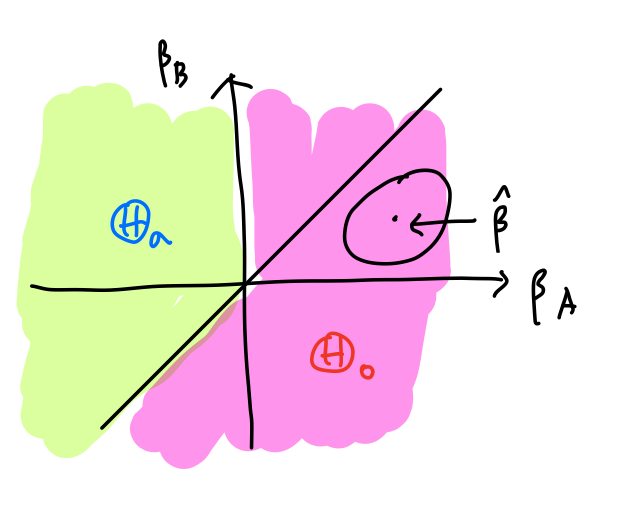
\includegraphics[width=.5\textwidth]{figures/hypo.png}
      \centering
      \caption{Null space $\Theta_0$ vs alternative space $\Theta_a$}
      \label{fig:hypo}
\end{figure}

If the test is to be carried out at the significance level $\alpha = 0.05$,
\begin{itemize}
\item If $A\hat{\beta}\in \Theta_0$, we do not reject $H_0$.
\item If $A\hat{\beta}\in \Theta_a$, we reject $H_0$ iff the 95\% confidence region of $\gamma$, $C_{0.95}$, does not intersect with the null space $\Theta_0$.
\end{itemize}
\ed

The process guarantees under the null hypothesis, the probability of rejection is less than the significance level. The area of $\hat{\beta}$ that results in rejecting the null hypothesis is drawed as a red area in Figure 2.

\begin{figure}[h]
      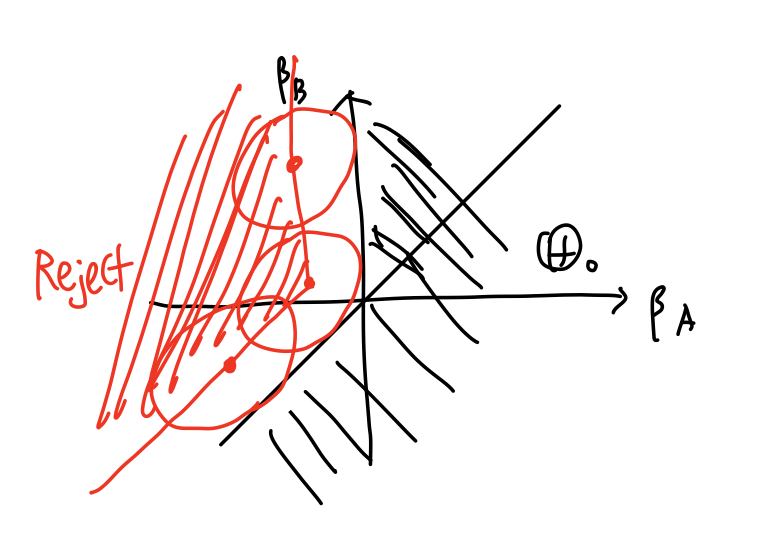
\includegraphics[width=.5\textwidth]{figures/reject.png}
      \centering
      \caption{Null space $\Theta_0$ vs alternative space $\Theta_a$}
      \label{fig:reject}
\end{figure}


\pr{5} (5 points) Which methods would you use for residual analysis?

\so

Let the following respectly as the pearson and deviance residual of the GLM model.
\begin{align*}
\gamma_{P,i} &= \frac{y_i-\mu_i}{\sqrt{V(\mu_i)}}\\
\gamma_{D,i} &= \text{sign}(y_i-\mu_i)\{2(y_i (\tilde{\theta}_i - \hat{\theta}_i) - b(\tilde{\theta}_i) + b(\hat{\theta}_i) )/\phi\}^{\frac{1}{2}}
\end{align*}
To proceed with the residual analysis, I would first plot the pearson and deviance residuals against fitted values to check if there are any systematic patterns left in the residuals. If the residuals show some curved pattern, it would indicate a lack-of-fit of the model.
Secondly, we can quickly compare the two residul values; if the two kinds of residuals are not quite similar to each other, the model may suffer from potential lack-of-fit. Finally, there is a \texttt{runs.test} function in R which tests against the null hypothesis that there are no systematic patterns in a sequence of random numbers, here the residuals. Applying two-sided runs test could be another way to check the lack-of-fit of the model.

Another usage of residual analysis is to find out outliers and influential points. To check leverage data points, plot the diagonal of hat matrix against the index of the points. An observation is suspected as a leverage point if $h_{ii} > 2p/n$, where $p$ is the number of coefficients in the model and $n$ sample size, respectively. To detect influential observations, use Cook’s distance and detect if the value is bigger than 1.

\ed

\pr{6} (5 points) Assume residual analysis indicates lack of fit and it seems that the effect of age is not linear. Provide two ways how you can proceed to allow for nonlinear effects of age in your model.

\so

I would consider adding polynomial terms of predictor age or adding interaction terms with other predictors. Also, if I would like to change the model structure, I would consider nonparametric smoothing methods. This might include any nonparametric regression method such as cubic smoothing splines, kernel regression, local linear regression and so on. For example, kernel regression would estimate the expected number of seizures given predictors with 
$$
\hat{m}(x) = \frac{\sum_{i=1}^n K(\frac{\|x-X_i\|}{h})Y_i}{\sum_{i=1}^n K(\frac{\|x-X_i\|}{h})}
$$
, where $h>0$ is the bandwidth parameder, and $K$ is a kernal function. As our response variable is count data, one could rescale the resulted estimator to get the final estimate.
\ed

\pr{7} (10 points) Now an investigator proposes to you to simply take log(counts+1) and then run a linear model with least squares. Can you fit this with a GLM? What are your considerations when responding to the request?

\so

To proceed with the fitting, I would regard $z_i = \log(y_i + 1)$ ($y_i$ : the counts of seizures) be our new response variable and run \textbf{multiple regression analysis} assuming errors independently follow normal distribution. This is exactly what the investigator wants us to do: run a linear model for log(counts+1) with least squares. Indeed, with this new variable $z_i$ following the normal distribution, applying multiple regression with least squares is also a version of GLM fitting. This is because normal distribution is also an exponential family and maximizing its likelihood is equivalent to minimizing the sum of squared errors problem.

On the other hand, if the investigator wants us to assume some distribution on $Y$ and regard $g(y) = \log(y+1)$ as a link function, I would say fitting this with a GLM model is somewhat inapprorpriate. Then fitting least squares to the log(counts+1) should be related to maximizing the likelihood of the observation based on $Y$'s distribution. But there is no concrete evidence that $Y$ follows such distribution (in the sense that $\max l(y;X) \Leftrightarrow \min (\log(y+1)-X\beta)^2$), especially in our case $Y$ taking discrete numbers. Another point is the fundamental of GLM setting. The GLM model assumes the linear model with predictors relates to the response variable via a link function, $\eta_i = g(\mu_i) = x_i^T\beta$. Here, the parameter of the link function is $\mu_i = \E(Y_i)$, not $y_i$. So, as investigator wants, applying $\log(y_i + 1)$ and fitting a model would not be the right way to proceed with GLM fitting.

\ed

\pr{8} (10 points) Consider the Gamma-Poisson model, where we assume that the counts $Y$ of seizures are Poisson distributed, $Y\sim \text{Poisson}(Z)$, where $Z$ itself is a patient-dependent random variable that is Gamma-distributed, $Z\sim \text{Gamma}(\kappa,\rho)$, with $E(Z)=\frac{\kappa}{\rho}$, $Var(Z)=\frac{\kappa}{\rho^2}$. Use a conditioning argument (note: do not use the Gamma density) to show:
\begin{align*}
E(Y)=\frac{\kappa}{\rho}, Var(Y)=\frac{\kappa(\rho+1)}{\rho^2}.
\end{align*}
Write the variance as a function of $\mu = E(Y)$ and $\rho$ and investigate its behavior for the case of small and large $\rho$.

\so

Note that if $X\sim \text{Poi}(\lambda)$, then $EX = \lambda, Var(X) = \lambda$. Since $Y\sim \text{Poisson}(Z)$, $E(Y|Z=z) = Var(Y|Z=z) = z$.
\begin{align*}
E(Y) &= E(E(Y|Z)) = E(Z) = \frac{\kappa}{\rho}\\
Var(Y) &= Var(E(Y|Z)) + E(Var(Y|Z))\\
	& = Var(Z) + E(Z) = \frac{\kappa}{\rho^2} + \frac{\kappa}{\rho} = \frac{\kappa(\rho+1)}{\rho^2}.
\end{align*}

Now let $\mu = \frac{\kappa}{\rho}$ then $Var(Y) = \frac{\kappa(\rho+1)}{\rho^2} = \mu \frac{\rho+1}{\rho}$. For large $\rho$, $Var(Y) \approx \mu$, thus modeling with poisson distribution without overdispersion would be approximately correct. When $\rho$ small, $Var(Y) = \mu +\frac{\mu}{\rho} \approx \frac{\mu}{\rho}$ gets bigger than $\mu$, and you will see the overdispersion (and approximately the overdispersion parameter would be $\frac{1}{\rho}$).
\ed

\pr{9} (5 points) The investigator informs you that there may be a subgroup of patients, who were included because they had a seizure a long time ago, but are actually not epileptic anymore. For these patients, there is no potential to observe any seizure, however we don’t know their identity. Extend your model accordingly and provide details of the extended model.

\so

To deal with the subgroup, I would extend the model allowing Zero-inflation. 
The probability distribution of number of seizures $Y$ can be expressed as 
$$\mathbf{P}(Y_i = y | X_i) = \alpha_i \mathbf{1}_{\{y = 0\}} + (1-\alpha_i) f(y,\mu_i)$$
, where $f(y,\mu_i)$ is the pmf of Poisson distribution with mean $\mu_i$ and $\alpha_i$ is interpreted as probability of structural zero.
To model $\alpha_i$, we will use binary regression with logit link, and estimate it using given predictors and unknown parameter $\gamma \in \mathbb{R}^6$. To model $\mu_i$, we will use the poisson regression with log link, and estimate it using given predictors and unknown parameter $\beta\in \mathbb{R}^6$.
\begin{itemize}
\item $\text{logit}(\alpha_i) = \tilde{\eta}_i = x_i^T\gamma$\ \ \&\ \ $\log(\mu_i) = \eta_i = x_i^T\beta$
\end{itemize}

\ed


\section{Data Analysis Solutions}

You can submit the answers of data analysis part by editing this latex file or generating another PDF file and combining it with this one. Please {\bf remove} the Data Analysis section in the final report and include GLM and Data Analysis Solutions sections only. 

I am attaching ipynb file together with py file. py file is just for reference and the content is same as ipynb file.

\pr{1} Describe your model. 

My final model is Ensemble of DLA3 model and VGG11 with Batch Normalization model. Here I will describe the detail of the model structure.

\begin{table}[h]
\begin{tabular}[\textwidth]{ | c | c | c | c | c | c  | c | c | c | }
\hline
Model & DLA3 & Dense121 & Resnet34 & Resnet50 & Vgg11 &  Vgg11bn & Vgg13 &  Vgg13bn \\
\hline
Train Acc &  0.9674 & 0.9424  & 0.9754  & 0.9826   & 0.9769 & 0.9861  & 0.9781 & 0.9583 \\
Val Acc & 0.9717 & 0.9571  & 0.9733 & 0.9762 & 0.9779  & \textbf{0.9846}  & 0.9754  & 0.9712 \\
\hline
\end{tabular}
\label{tab:models}
\caption{Training and Validation accuracies for different models}
\end{table}


First of all, to choose the best model for this 3-class image classification problem, I did a simple experiment comparing models' performance. Here I considered the following models:  DLA3, Dense121, Resnet34, Resnet50, Vgg11,  Vgg11bn, Vgg13,  Vgg13bn.
Before mentioning the implementation details for each model, I would first talk about the experiment. I compared the training and validation accuracy results after 10 epochs with batch size 100 and learning rate 0.01. Table 1 shows the results. As we can see, VGG11 model with batch normalization (Vgg11bn) model showed the best accuracy (with validation accuracy 0.9846) among the candidates, so I proceeded with the model. 
Later, to improve the performance, I considered ensemble modeling. So I chose resnet50 model to ensemble with vgg11bn model because it showed the best performance other than vgg models.

All but DLA3 model are \texttt{torchvision.models} built-in models. For DLA3 model, I used the model used for classifying CIFAR10 dataset from the github source provided by this link: \href{https://github.com/kuangliu/pytorch-cifar}{\color{blue}DLA3 model source}. I copied dla.py file and used the code like the following code. 
\begin{verbatim}
from dla import DLA
model = DLA(num_classes=3)
\end{verbatim}
 Other than this, since torchvision built-in models are aim to built for classifying Imagenet datasets, I had to modify the models seperately to fit the image sizes and work for our dataset. The details are following.

\begin{itemize}
\item For all the models, I changed the last fc layer number of ouput classes from 1000 to 3. Here is the example applied for resnet50 model
\begin{verbatim}
resnet50.classifier = nn.Linear(2048,3)
resnet50.fc = nn.Linear(2048,3)
\end{verbatim}
\item For all the models, I changed the first convolution layer. It originally takes kernel size (7, 7), and stride (2, 2), padding (3, 3). For our imageset, after the layer it becomes (64,16,16). I changed it to take kernel size (3,3), stride (1,1), padding (1,1), whose ouput size becomes (64, 32, 32).
\item For vgg models, I tried both the vgg model and vgg model with batch normalization. To add this additional regularization, I added BatchNorm2d layer after each Conv2d layer, which is implemented as follows.
\begin{verbatim}
bn = []
for layer in vgg11bn.features:
    bn += [layer]
    if isinstance(layer, nn.Conv2d):
        bn += [nn.BatchNorm2d(layer.out_channels)]
vgg11bn.features = nn.Sequential(*bn)
\end{verbatim}
\end{itemize} 

Detailed architecture of my Vgg11bn model is that it takes [64, 'M', 128, 'M', 256, 256, 'M', 512, 512, 'M', 512, 512, 'M'] layers, each number implying the number of out channels and 'M' implying Maxpooling layer. Convolution layers take kernel size (3, 3), stride (1, 1), padding (1, 1), which does not change the image size. Maxpooling layers take kernel size 2, stride 2, padding 0, which reduces the image size to be half. After 5 Maxpooling layers, the image gets its output size of (512,1,1). Then the final classifier consists of Fully connected linear layer with two sets of [out features 4096, ReLU, Dropout] layers and then Linear layer of final number of out features 3.

Our resnet50 model architecture consists of 4 Sequential layers after which the image size reduces to its half so it becomes (2048, 2,2). Number of channels increase as [64, 128, 256, 512, 1024, 2048] and the final fully connected layer is a Linear layer connecting (2048, 3).


% 모델 설명


\pr{2} Generate a plot to visualize the batch loss during training. (Y-axis: loss, X-axis: iteration). 

\begin{figure}[h]
      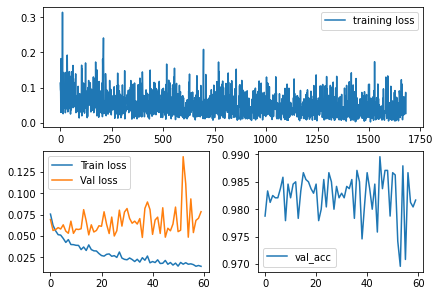
\includegraphics[width=.7\textwidth]{figures/vgg11bn_result.png}
      \centering
      \caption{(top) Batch loss (bottom) Loss and accuracy for 60 epochs; VGG11bn model}
      \label{fig:vggrslt}
\end{figure}

\begin{figure}[h]
      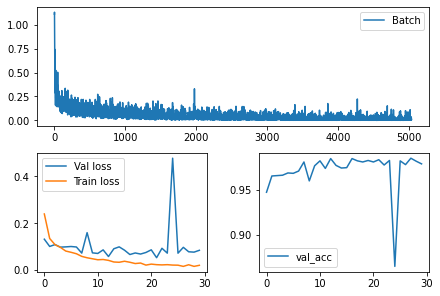
\includegraphics[width=.7\textwidth]{figures/res50result.png}
      \centering
      \caption{(top) Batch loss (bottom) Loss and accuracy for 30 epochs; resnet50 model}
      \label{fig:resrslt}
\end{figure}

\begin{figure}[h]
      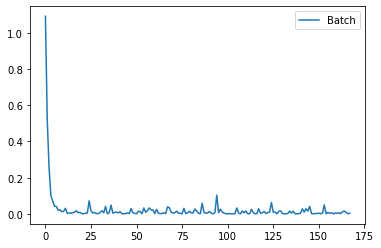
\includegraphics[width=.5\textwidth]{figures/esb_batch.png}
      \centering
      \caption{Training batch loss for ensemble model}
      \label{fig:esbbatch}
\end{figure}

\begin{figure}[h]
      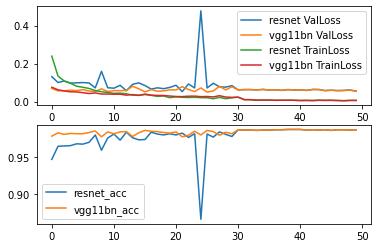
\includegraphics[width=.7\textwidth]{figures/ensemble_result.png}
      \centering
      \caption{Loss and accuracy of resnet50 and vgg11bn followed by the ensemble model result (from epoch 25)}
      \label{fig:esbrslt}
\end{figure}

%Esble result
Figure \ref{fig:vggrslt} and \ref{fig:resrslt} respectively shows the result for VGG11bn model and Resnet50 model. For Vgg11bn model, the top figure shows the training batch loss for 10 epoch, total of 1680 batch losses. For resnet50 model the top figure is training batch loss for 30 epochs. For both result, batch loss (blue line in bottom left figures) tend to keep decrease, while vallidation loss and validation accuracy does not improve at some point. It could be interpreted as an existence of overfitting. So I applied Early stopping and chose epoch 25 result to feed the ensemble model. As one can see, the validation performances are not consistent for both models. It works relatively well for some epochs while comparatively poorly for others. To make it stabilize, I used Ensemble model to generate my final model. Details will be explained at part 5. Figure \ref{fig:esbbatch} shows the training batch loss of the ensemble model. I only plotted the first epoch (168 batches) because it keeps showing the consistent trend we can observe from the figure and thus plotting after 1 epoch draws almost constant line near 0. What is surprising is how fast it learns, even after 5 batches (not epochs) it stabilizes. This is due to we already use weights trained from vgg11bn and resnet50 models. Figure \ref{fig:esbrslt} shows more astonishing result of ensemble training. I plotted each of resnet50 and vgg11bn model's loss and accuracies followed by those of ensemble training from epoch 26. The figure shows the clear result of ensemble results' consistency. The validation performance has stabilized and it shows consistent result. This clearly shows the power of ensemble training!

\pr{3} Report the classification accuracy on the train and val sets.

\begin{table}[h]
\centering
\begin{tabular}[\textwidth]{ | c | c | c | c | }
\hline
Model & Resnet50 & Vgg11bn & Ensemble \\
\hline
Train Acc &  0.9923 & 0.9902  & \textbf{0.9971} \\
Val Acc & 0.9817 & 0.9867  & \textbf{0.9879} \\
\hline
\end{tabular}
\label{Tab:acc}
\caption{Training and Validation accuracy result}
\end{table}

Table 2 is the final accuracy of our models. Models are trained using learning late 0.01 and batch size 100. Our final model is the ensemble result of Resnet50 and Vgg11bn model after 9 epochs. The final validation and training accuracies are 0.9879 for validation and 0.9971 for training set.
%table for three models


\pr{4} Report the training parameters: number of epochs, optimizer and related parameters (learning rate, penalty, momentum etc).

Training parameters are as follows:

I used epoch 25 for training Vgg11bn model and Resnet50 model and epoch 8 for the ensemble model. These number of epochs are chosen to be when the model yeild sufficiently good performance. As we can see in the Figure \ref{fig:vggrslt}, longer epochs does not yield the better model, but there occurs an overfitting. Below codes show the optimizer and related parameters.

\begin{lstlisting}[language=Python]
optimizer = optim.SGD(model.parameters(), lr=0.01, momentum=0.9, weight_decay=5e-4) 
scheduler = torch.optim.lr_scheduler.CosineAnnealingLR(optimizer, T_max=200)
\end{lstlisting}


\pr{5} Report any techniques you used to improve the performance. Example: data augmentation, data normalization, learning rate tuning, etc. 

\begin{itemize}
\item Model Comparison

As explained in part 1 table 1, I compared the performance of several state-of-art architectures from the beginning. From this step, I chose vgg11 with batch normalization model shows the best performance for our task among 8 different model structures.

\item Ensemble Model

Figure \ref{fig:esbrslt} shows how ensemble model stabilizes the prediction performance. I emplemeted my ensemble model to combine the vgg11bn and resnet50 model results. To proceed, I removed the final fully connected layer from each and created new classifier taking inputs from 2046(resnet) + 4096 (vgg11bn) last channels. The code is as follows.

\begin{lstlisting}[language=Python]
class MyEnsemble(nn.Module):
    def __init__(self, modelA, modelB, nb_classes=3):
        super(MyEnsemble, self).__init__()
        self.modelA = modelA #modelA : resnet50
        self.modelB = modelB #modelB : VGG11+bn
        # Remove last linear layer
        self.modelA.fc = nn.Identity()
        self.modelB.classifier[6] = nn.Identity()
        
        # Create new classifier
        self.classifier = nn.Linear(2048+4096, nb_classes)
        
    def forward(self, x):
        x1 = self.modelA(x.clone()) 
        x1 = x1.view(x1.size(0), -1)
        x2 = self.modelB(x)
        x2 = x2.view(x2.size(0), -1)
        x = torch.cat((x1, x2), dim=1)
        
        x = self.classifier(nn.functional.relu(x))
        return x
\end{lstlisting}

Then we can use MyEnsemble model by \texttt{MyEnsemble(resnet50, vgg11bn)}. 

\item Early Stopping

As one can see in the figure \ref{fig:vggrslt}, training loss tends to keep decreasing as training longer, but validation loss or accuracy does not increase a lot and rather it fluctuates.
To avoid overfitting, I applied early stopping so that model can stop learning if it shows sufficiently good performance. As a result, I chose epoch 25 for vgg11bn and resnet50 models. 

\item Data augmentation and normalization.

I used \texttt{RandomCrop, RandomHorizontalFlip} methods for the data augmentation method. Also, I normalized the images before using it.

To normalize the data, compute the mean and standard deviation after loading images without random transforms and nomalizations. Here we get \texttt{mean=[0.8260, 0.6706, 0.7601], std=[0.0977, 0.1722, 0.1293]}. Then we assign the transforms to training and test loaders as the following code .

\begin{lstlisting}[language=Python]
normalize = transforms.Normalize(mean=[0.8260, 0.6706, 0.7601],
                                 std=[0.0977, 0.1722, 0.1293])
trans_train = transforms.Compose([
        transforms.RandomCrop(32, padding=4),
        transforms.RandomHorizontalFlip(),
        transforms.ToTensor(),
        normalize ])
\end{lstlisting}

\item Learning Rate tuning

Due to the limitation of colab usage, I compared 10-epochs-results of two learning rate 0.1 and 0.01 for VGG11 with batch normalization model. Figure \ref{fig:lr} shows the mean training loss per each epoch graph. Clearly, learning rate matters and learning rate 0.01 works much faster and better.

\begin{figure}
      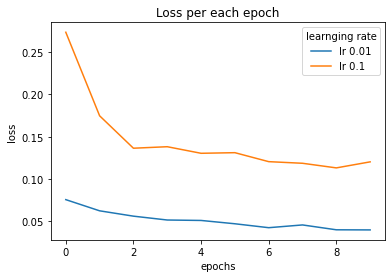
\includegraphics[scale=0.6]{figures/lr_experiment.png}
      \centering
      \caption{Traning loss with different learning rate}
      \label{fig:lr}
\end{figure}

\item Batch normalization

For vgg11bn model, I added batch normalization after each convolution layers to regularize the result using the following code.

\begin{lstlisting}[language=Python]
bn = []
for layer in vgg11bn.features:
    bn += [layer]
    if isinstance(layer, nn.Conv2d):
        bn += [nn.BatchNorm2d(layer.out_channels)]
vgg11bn.features = nn.Sequential(*bn)
\end{lstlisting}

\end{itemize}

\pr{6} Provide your prediction on the test set in a csv file. 

%----------------------------------------------------------------

\end{document}


%%%%%%%%%%%%%%%%%%%%%%%%%%%%%%%%%%%%%%%%%%%%%%%%%%%%%%%%%%%%%%%%%
%%%%%%%%%%%%%%%%%%%%%%%%%%%%%%%%%%%%%%%%%%%%%%%%%%%%%%%%%%%%%%%%%
%%%%%%%%%%%%%%%%%%%%%%%%%%%%%%%%%%%%%%%%%%%%%%%%%%%%%%%%%%%%%%%%%
